
\section{stack canaries}
\subsection{in code}
\usetikzlibrary{decorations.pathreplacing,decorations.pathmorphing}

\begin{frame}<1>[fragile,label=reCanary]{compiler generated code}
\lstset{
    language=myasm,
    style=smaller,
    moredelim={**[is][\btHL<2|handout:0>]{~2~}{~end~}},
    moredelim={**[is][\btHL<3|handout:0>]{~3~}{~end~}},
}
\vspace{-.25cm}
\begin{lstlisting}
    pushq %rbx
    sub $0x20,%rsp
/* copy value from thread-local storage */
    mov $0x28,%ebx
    mov %fs:(%rbx),%rax
/* onto the stack */
    mov %rax,0x18(%rsp)
/* clear register holding value */
    ~2~xor %eax, %eax~end~
    ...
    ...
/* copy value back from stack */
    mov 0x18(%rsp),%rax
/* xor to compare */
    ~2~xor %fs:(%rbx),%rax~end~
/* if result non-zero, do not return */
    jne call_stack_chk_fail
    ret
call_stack_chk_fail:
    call __stack_chk_fail
\end{lstlisting}
\begin{tikzpicture}[overlay,remember picture]
\begin{pgfonlayer}{fg}
    \coordinate (stack tl) at ([xshift=-4cm,yshift=-1cm]current page.north east);
    \coordinate (stack tr) at ([xshift=-.5cm,yshift=-1cm]current page.north east);
    \draw[very thick] (stack tl) -- ++(0, -6) coordinate (stack bl);
    \draw[very thick] (stack tr) -- ++(0, -6) coordinate (stack br);
    \draw[very thick,decorate,decoration={zigzag}] (stack tl) -- (stack tr);
    \draw[very thick,decorate,decoration={zigzag}] (stack bl) -- (stack br);
\end{pgfonlayer}
\path[draw,thick,fill=yellow!20] (stack tl) ++(0cm, -1cm) coordinate (ra tl) rectangle ++(3.5, -.5) coordinate (ra br)
    node [midway] {return address};
\coordinate (ra bl) at (ra tl |- ra br);
\path[draw,thick,fill=red!20] (ra bl) rectangle ++(3.5, -.5) coordinate (can br)
    node [midway] {stack canary};
\coordinate (can bl) at (ra tl |- can br);
\path[draw,thick,fill=green!20,align=center,font=\small] (can bl) rectangle ++(3.5, -2) 
    node [midway] {function's \\ arrays \\ and other \\ temporaries};
\begin{pgfonlayer}{fg}
    \begin{visibleenv}<2>
    \node[fill=white,draw=red,very thick,anchor=east,align=center] at ([xshift=-1cm]current page.east) {
        trying to avoid info disclosure: \\
        get canary value out of \%rax \\
        as soon as possible
    };
    \end{visibleenv}
\end{pgfonlayer}
\end{tikzpicture}
\end{frame}



\subsection{general operation}
\usetikzlibrary{arrows.meta}

\begin{frame}[fragile,label=returnToStackCanaryPic]{stack canary}
\begin{tikzpicture}
% FIXME:
\tikzset{
    stackBox/.style={very thick},
    onStack/.style={thick},
    xscale=1.3,
}
\draw[stackBox] (0, 0) rectangle (10, -6);
\draw[thick,-Latex] (10.25,-5) -- (10.25, -1) node [midway, below, sloped] {increasing addresses};
\node[at={(5, 0.1)},anchor=south] { highest address (stack started here)};
\node[at={(5, -6.1)},anchor=north] { lowest address (stack grows here)};

\draw[onStack] (0, -.25) rectangle (10, -1.25) node[midway,align=center,font=\small] (stackAddr)
     {return address for {\tt vulnerable}: \\
     \only<1>{\fontsize{10}{11}\selectfont\tt\color{black}37 fd 40 00  00 00 00 00 (0x40fd37)}
     \only<2>{\fontsize{10}{11}\selectfont\tt\bfseries\color{red}70 fd ff ff  ff ff 00 00 (0x7fff ffff fd70)}};
\draw[onStack,fill=black!20] (0, -1.25) rectangle (10, -1.75) node[midway,align=center,font=\small] {canary: \only<1>{\tt b1 ab bd e8 31 15 df 31}\only<2>{\color{red}{\tt ?? ?? ?? ?? ?? ?? ??}}};
\draw[onStack,fill=black!20] (0, -1.75) rectangle (10, -2.25) node[midway,align=center,font=\small] {unused space (12 bytes)};
\draw[onStack,fill=blue!20] (0, -2.25) rectangle (10, -5.25) node[midway,align=center,font=\small] {buffer (100 bytes)};

\draw[onStack] (0, -5.25) rectangle (10, -6) node[midway,align=center,font=\small] {return address for {\tt scanf}};

\begin{visibleenv}<2>
\draw[-Latex,red,ultra thick] ([yshift=2.5mm]stackAddr.south east) -- ++(.25cm,0cm) |- (0.25, -5);
\node[anchor=south west,red] at (0.25, -4.75) {
    machine code for the attacker to run
};
\end{visibleenv}

\end{tikzpicture}
\end{frame}



\subsection{requirements and how they can fail to be met}

\begin{frame}<1>[label=stackCanHopes]{stack canary hopes}
    \begin{itemize}
    \item \myemph<2>{overwrite return address $\implies$ overwrite canary}
    \item \myemph<3>{canary is secret}
    \end{itemize}
\end{frame}


 % FIXME: repeat slide with highlites

\subsection{how glibc generates canaries}

\begin{frame}{good choices of canary}
\begin{itemize}
\item \myemph{random} --- guessing should not be practical
    \begin{itemize}
    \item not always --- sometimes static or only $2^{15}$ possible
    \end{itemize}
\item GNU libc: canary contains:
\vspace{.5cm}
    \item leading {\tt \textbackslash 0} (string terminator)
        \begin{itemize}
        \item {\tt printf \%s} won't print it
        \item copying a C-style string won't write it
        \end{itemize}
    \item a newline
        \begin{itemize}
        \item read line functions can't input it
        \end{itemize}
    \item {\tt \textbackslash xFF}
        \begin{itemize}
        \item hard to input?
        \end{itemize}
\end{itemize}
\end{frame}


\subsection{GCC and canaries}

\begin{frame}{stack canaries implementation}
    \begin{itemize}
    \item ``StackGuard'' --- 1998 paper proposing strategy
    \item GCC: command-line options
        \begin{itemize}
        \item {\tt -fstack-protector} 
        \item {\tt -fstack-protector-strong} 
        \item {\tt -fstack-protector-all}
        \item one of these often default
        \item three differ in how many functions are `protected'
        \end{itemize}
    \item Microsoft C/C++ compiler: {\tt /GS}
        \begin{itemize}
        \item on by default
        \end{itemize}
    \end{itemize}
\end{frame}




\subsection{canary costs}

\begin{frame}{stack canary overheads}
    \begin{itemize}
    \item less than 1\% runtime if added to ``risky'' functions
        \begin{itemize}
        \item functions with character arrays, etc.
        \end{itemize}
    \item large overhead if added to all functions
        \begin{itemize}
        \item StackGuard paper: 5--20\%?
        \end{itemize}
    \item similar space overheads
    \vspace{.5cm}
    \item (for typical applications)
        \begin{itemize}
        \item could be much worse: tons of `risky' function calls
        \end{itemize}
    \end{itemize}
\end{frame}




\subsection{overall pros/cons}

\begin{frame}{stack canaries pro/con}
    \begin{itemize}
        \item pro: no change to calling convention
        \item pro: recompile only --- no extra work
        \item con: can't protect existing executable/library files (without recompile)
        \item con: \myemph<2>{doesn't protect against many ways of exploiting buffer overflows}
        \item con: \myemph<3>{vulnerable to information leaks}
    \end{itemize}
\end{frame}




\subsection{stack canary summary}

\begin{frame}{stack canary summary}
    \begin{itemize}
    \item stack canary --- simplest of many \myemph{mitigations}
    \item key idea: detect corruption of return address
    \item assumption: if return address changed, so is adjacent token
    \item assumption: attacker can't learn true value of token
        \begin{itemize}
        \item often possible with memory bug
        \end{itemize}
    \vspace{.5cm}
    \item later: workarounds to break these assumptions
    \end{itemize}
\end{frame}




\subsection{noncontiguous overwrites}
\againframe<2>{stackCanHopes}
\usetikzlibrary{decorations.pathreplacing,decorations.pathmorphing}

\begin{frame}[fragile,label=stackNonContig]{non-contiguous overwrites}
\begin{lstlisting}[style=small]
void vulnerable() {
  int scores[8]; bool done = false;
  while (!done) {
    cout << "Edit which score? (0 to 7) ";
    int i;
    cin >> i;
    /* Oops!
       sizeof(scores) is 4 * sizeof(int) */
    if (i < 0 || i >= sizeof(scores))
      continue;
    cout << "Set to what value?" << endl;
    cin >> scores[i];
    ...
  }
  ...
}
\end{lstlisting}
\begin{tikzpicture}[overlay,remember picture,y=1.25cm]
\begin{pgfonlayer}{fg}
\coordinate (stack tl) at ([xshift=-4cm,yshift=-1cm]current page.north east);
\coordinate (stack tr) at ([xshift=-.5cm,yshift=-1cm]current page.north east);
\draw[very thick] (stack tl) -- ++(0, -6) coordinate (stack bl);
\draw[very thick] (stack tr) -- ++(0, -6) coordinate (stack br);
\draw[very thick,decorate,decoration={zigzag}] (stack tl) -- (stack tr);
\draw[very thick,decorate,decoration={zigzag}] (stack bl) -- (stack br);
\end{pgfonlayer}
\path[draw,thick,fill=yellow!20] (stack tl) ++(0cm, -1cm) coordinate (ra tl) rectangle ++(3.5, -.5) coordinate (ra br)
    node [midway] {return address};
\coordinate (ra bl) at (ra tl |- ra br);
\path[draw,thick,fill=red!20] (ra bl) rectangle ++(3.5, -.5) coordinate (can br)
    node [midway] {stack canary};
\coordinate (can bl) at (ra tl |- can br);
\foreach \x/\idx in {0/7, 1/6, 2/5, 3/4, 4/3, 5/2, 6/1, 7/0} {
    \path[draw,thick,fill=green!20,align=center,font=\small] (can bl) ++ (0, -\x * 0.25)
        rectangle ++(3.5, -0.25)  node[midway,font=\tt\fontsize{9}{10}\selectfont]{scores[\idx]};
}
\path[fill=violet!30,opacity=0.5] (can bl) ++ (0, -8 * 0.25) rectangle ++(3.5, -1.5) 
    node[midway,font=\fontsize{9}{10}\selectfont,align=center] {stack grows here for \\ calls to cin/cout \\ methods};
\end{tikzpicture}
\end{frame}


%FIXME: polls entry for exercise
\usetikzlibrary{decorations.pathreplacing,decorations.pathmorphing}

\begin{frame}[fragile,label=stackNonContigEx]{exercise: non-contiguous overwrites}
\begin{lstlisting}[style=small]
void vulnerable() {
  int scores[8]; bool done = false;
  while (!done) {
    cout << "Edit which score? (0 to 7) ";
    int i;
    cin >> i;
    /* Oops!
       sizeof(scores) is 4 * sizeof(int) */
    if (i < 0 || i >= sizeof(scores))
      continue;
    cout << "Set to what value?" << endl;
    cin >> scores[i];
    ...
  }
  ...
}
\end{lstlisting}
\begin{tikzpicture}[overlay,remember picture,y=1.25cm]
\begin{pgfonlayer}{fg}
\coordinate (stack tl) at ([xshift=-4cm,yshift=-1cm]current page.north east);
\coordinate (stack tr) at ([xshift=-.5cm,yshift=-1cm]current page.north east);
\draw[very thick] (stack tl) -- ++(0, -6) coordinate (stack bl);
\draw[very thick] (stack tr) -- ++(0, -6) coordinate (stack br);
\draw[very thick,decorate,decoration={zigzag}] (stack tl) -- (stack tr);
\draw[very thick,decorate,decoration={zigzag}] (stack bl) -- (stack br);
\end{pgfonlayer}
\path[draw,thick,fill=yellow!20] (stack tl) ++(0cm, -1cm) coordinate (ra tl) rectangle ++(3.5, -.5) coordinate (ra br)
    node [midway] {return address};
\coordinate (ra bl) at (ra tl |- ra br);
\path[draw,thick,fill=red!20] (ra bl) rectangle ++(3.5, -.5) coordinate (can br)
    node [midway] {stack canary};
\coordinate (can bl) at (ra tl |- can br);
\foreach \x/\idx in {0/7, 1/6, 2/5, 3/4, 4/3, 5/2, 6/1, 7/0} {
    \path[draw,thick,fill=green!20,align=center,font=\small] (can bl) ++ (0, -\x * 0.25)
        rectangle ++(3.5, -0.25)  node[midway,font=\tt\fontsize{9}{10}\selectfont]{scores[\idx] (4 byte)};
}
\path[fill=violet!30,opacity=0.5] (can bl) ++ (0, -8 * 0.25) rectangle ++(3.5, -1.5) 
    node[midway,font=\fontsize{9}{10}\selectfont,align=center] {stack grows here for \\ calls to cin/cout \\ methods};
\node[draw=red,anchor=south,very thick,align=center,fill=white] at ([xshift=-2cm,yshift=.25cm]current page.south) {
    exercise: to set return address to 0x123456789, \\
    set what scores to what values?
};
\end{tikzpicture}
\end{frame}

\begin{frame}
\begin{tabular}{l}
\tt 0x123456789 \\
\tt 0x0000 0001 2345 6789 \\
\tt 89 67 45 23 01 00 00 00 \\
\tt [89 67 45 23] [01 00 00 00] \\
\tt 0x2345678 0x1
\end{tabular}
\end{frame}


\subsection{information disclosure}
\againframe<3>{stackCanHopes}
\subsubsection{examples}
\begin{frame}[fragile,label=infoDisc1a]{information disclosure (1a)}
\lstset{
    language=C++,
    style=small
}
\begin{lstlisting}
void vulnerable() {
    int value;
    for (;;) {
        command = ReadInput();
        if (command == "set") {
            value = ReadIntInput();
        } else if (command == "get") {
            printf("%d\n", value);
        } else if ...
    }
}
\end{lstlisting}
\begin{itemize}
\item ``get'' command: can read \myemph{uninitialized value}
\item example: when I compiled this, \texttt{value} was stored on the stack
\end{itemize}
\end{frame}

\begin{frame}[fragile,label=infoDisc1b]{information disclosure (1b)}
\lstset{
    language=C++,
    style=smaller
}
\begin{lstlisting}
void vulnerable() {
    int value;
    ...
        } else if (command == "get") {
            cout << value << endl;
        }
    ...
}
void leak() {
    int secrets[] = { 
        12345678, 23456789, 34567890,
        45678901, 56789012, 67890123,
    };  
    do_something_with(secrets);
}
int main() {leak(); vulnerable();}
\end{lstlisting}
\begin{tikzpicture}[overlay,remember picture]
\node[draw,very thick,anchor=north east,align=left] at ([xshift=-.25cm,yshift=-.25cm]current page.north east) {
running this program \\
(input in bold): \\
\tt \textbf{get} \\
\tt 67890123
};
\end{tikzpicture}
\end{frame}

\begin{frame}[fragile,label=infoDisc2]{information disclosure (2)}
\lstset{
    language=C,
    style=small
}
\begin{lstlisting}
void process() {
    char buffer[8] = "\0\0\0\0\0\0\0\0";
    char c = ' ';
    for (int i = 0; c != '\n' && i < 8; ++i) {
        c = getchar();
        buffer[i] = c;
    }
    printf("You input %s\n", buffer);
}
\end{lstlisting}
\begin{itemize}
\item input \verb|aaaaaaaa|
\item output \verb|You input aaaaaaaa|{\it (whatever was on stack)}
\end{itemize}
\end{frame}

\begin{frame}[fragile,label=infoDisc3]{information disclosure (3)}
\lstset{
    language=C,
    style=small,
}
\begin{lstlisting}
struct foo {
    char buffer[8];
    long *numbers;
};

void process(struct foo* thing) {
    ...
    scanf("%s", thing->buffer);
    ...
    printf("first number: %ld\n", thing->numbers[0]);
}
\end{lstlisting}
\begin{itemize}
\item input: {\tt aaaaaaaa}\textit{(address of canary)}
    \begin{itemize}
    \item address on stack \textit{or} where canary is read from in thread-local storage
    \end{itemize}
\end{itemize}
\end{frame}



\subsubsection{exercise}
\begin{frame}{recall: ASLR}
    \begin{itemize}
    \item easlier mentioned ASLR (address space layout randomization)
    \item for stack: choose secret starting address for stack
    \vspace{.5cm}
    \item info disclosure bugs are a big problem for this!
    \end{itemize}
\end{frame}

\begin{frame}[fragile,label=infoDiscEx]{exercise}
\begin{tikzpicture}
\node (first) {
\begin{lstlisting}[language=C,style=smaller]
struct point {
    int x, y, z;
};
\end{lstlisting};
};
\node[anchor=north west] at (first.north east) {
\begin{lstlisting}[language=C,style=smaller]
struct point *p;
...
    if (command == "get") { 
        /* 'p' could be uninitialized */
        printf("%d,%d,%d\n", p->x, p->y, p->z);
    } ...
...
\end{lstlisting}
};
\end{tikzpicture}
\vspace{-.25cm}
\begin{itemize}
\item Which initial value for \texttt{p} (``left over'' from prior use of register, etc.) would be most useful for figuring out the address of the stack pointer?
\begin{itemize}
\item A. \texttt{p} is an invalid pointer and accessing it will crash the program
\item B. \texttt{p} points to space on the stack that is currently unallocated, but last contained an input buffer
\item C. \texttt{p} points to a struct allocated on the heap
\item D. \texttt{p} points to space on the stack that currently holds a return address
\item E. \texttt{p} points to space on the stack that is currently unallocated, but last contained a pointer to the last used byte of an input buffer on the stack
\end{itemize}
\end{itemize}
\end{frame}


\subsubsection{avoiding?}
\againframe<2>{reCanary}

% FIXME: exercise: using info disclosure bug?

\section{shadow stacks}
\usetikzlibrary{arrows.meta,shapes.multipart,patterns}

\begin{frame}{intuition: shadow stacks}
    \begin{itemize}
    \item problem with stack: easy to leak address/values because used for lots of data
    \vspace{.5cm}
    \item goal: keep sensitive data in \textbf{separate region}
        \begin{itemize}
        \item easier to kepe address secret?
        \end{itemize}
    \vspace{.5cm}
    \item can use this for (stronger?) alternative to stack canaries
    \end{itemize}
\end{frame}

\tikzset{
    stackBox/.style={very thick},
    onStack/.style={thick},
    frameOne/.style={fill=blue!15},
    frameTwo/.style={fill=red!15},
    markLine/.style={blue!50!black},
    markLineB/.style={red!90!black},
    hiLine/.style={red!90!black},
}
\begin{frame}{shadow stacks}
    \begin{tikzpicture}
    \tikzset{
        mainSt/.style={fill=blue!20},
        otherSt/.style={fill=yellow!20},
        every node/.style={font=\small,align=center},
    }
    \draw[stackBox,mainSt] (0, 0) rectangle (5, -6);
    \node[anchor=south] at (2.5, 0) { main stack @ \\ \texttt{0x7 0000 0000}};
    \begin{scope}[yshift=-.25cm]
    \draw[onStack] (0, 0) rectangle (5, -1.5) node[midway] {local variables for \texttt{foo}};
    \draw[onStack] (0, -1.5) rectangle (5, -2) node[midway] {arguments for \texttt{bar}};
    \draw[onStack] (0, -2) rectangle (5, -3.5) node[midway] {local variables for \texttt{bar}};
    \draw[onStack] (0, -3.5) rectangle (5, -4.0) node[midway] {arguments for \texttt{baz}};
    \draw[red,very thick,Latex-] (5.25, -4.0) -- ++(.5, 0) node[right] {stack pointer};
    \end{scope}
    \node[anchor=south] at (9, 0) { `shadow' stack @ \\ \texttt{0x8 0000 0000}};
    \draw[stackBox,otherSt] (6.5, 0) rectangle (11.5, -3);
    \begin{scope}[yshift=-.25cm,xshift=6.5cm]
    \draw[onStack] (0, 0) rectangle (5, -0.5) node[midway] {return address for \texttt{foo}};
    \draw[onStack] (0, -0.5) rectangle (5, -1) node[midway] {return address for \texttt{bar}};
    \draw[onStack] (0, -1) rectangle (5, -1.5) node[midway] {return address for \texttt{baz}};
    \draw[red,very thick,Latex-] (5.25, -1.5) -- ++(.5, 0) node[right] {shadow \\stack pointer};
    \end{scope}
    \end{tikzpicture} 
\end{frame}

\begin{frame}{implementing shadow stacks}
    \begin{itemize}
    \item bigger changes to compiler than canaries
    \item more overhead to call/return from function
    \item most commonly: store return address twice
    \end{itemize}
\end{frame}

\begin{frame}[fragile,label=shadowStackx8664v1]{shadow stacks on x86-64 (1)}
\begin{itemize}
\item idea 1: dedicate \%r15 as shadow stack pointer, \\
      copy RA to shadow stack pointer in function prologue
\end{itemize}
\begin{lstlisting}[language=myasm]
function:
    movq (%rsp), %rax    // RAX <- return address
    addq $-8, %r15       // R15 <- R15 - 8
    movq %rax, (%r15)    // M[R15] <- RAX
    ...
    movq (%rsp), %rdx     // RDX <- return address
    cmpq %rdx, (%r15)    
    jne CRASH_THE_PROGRAM // if RDX != M[R15] goto CRASH_THE_PROGRAM
    add $8, %r15          // R15 <- R15 - 8
    ret
\end{lstlisting}
\end{frame}

\begin{frame}[fragile,label=shadowStackx8664v2]{shadow stacks on x86-64 (2)}
\begin{itemize}
\item idea 2: dedicate \%r15 as shadow stack pointer, \\
      avoid normal call/return instruction
\end{itemize}
\begin{lstlisting}[language=myasm]
    addq $-8, %r15
    leaq after_call(%rip), %rax
    movq %rax, (%r15)
    jmp function
after_call:

function:
    ...
    addq $8, %r15        // R15 <- R15 + 8
    jmp *-8(%r15)        // jmp M[R15-8]
\end{lstlisting}
\end{frame}

\begin{frame}[fragile,label=actShadowStack]{Android/AArch64 shadow stacks (1)}
   \begin{itemize}
    \item {\tiny via \url{https://clang.llvm.org/docs/ShadowCallStack.html} (see also {\url{https://security.googleblog.com/2019/10/protecting-against-code-reuse-in-linux_30.html}})}
    \item dedicate register \texttt{x18} to shadow stack pointer
        \begin{itemize}
        \item x30 = return address (after ARM's call instruction (bl))
        \end{itemize}
    \item ARM call instruction saves return address in register\ldots
    \end{itemize}
\begin{tikzpicture}
\node[draw,label={with shadow stack}] (code1) {
\begin{lstlisting}[language={},style=script]
str     x30, [x18], #8      
stp     x29, x30, [sp, #-16]!
mov     x29, sp
bl      bar
add     w0, w0, #1
ldp     x29, x30, [sp], #16
ldr     x30, [x18, #-8]!
ret
\end{lstlisting}
};
\node[anchor=north east,draw,label={without}] (code2) at (code1.north west) {
\begin{lstlisting}[language={},style=script]
stp     x29, x30, [sp, #-16]!
mov     x29, sp
bl      bar
add     w0, w0, #1
ldp     x29, x30, [sp], #16
ret
\end{lstlisting}
};
\end{tikzpicture}
\end{frame}

\begin{frame}{Android/AArch64 shadow stacks (2)}
    \begin{itemize}
    \item \texttt{-fsanitize=shadowcallstack}
    \item supported on 64-bit ARM and RISC V only
    \vspace{.5cm}
    \item ``An x86\_64 implementation was evaluated using Chromium and was found to have critical performance and security deficiencies''
    \end{itemize}
\end{frame}


\subsection{Intel's hardware support?}
\begin{frame}{Intel CET shadow stacks}
    \begin{itemize}
    \item recent Intel processor extension adds shadow stacks
        \begin{itemize}
        \item ``Control-flow Enforcement Technology''
        \end{itemize}
    \vspace{.5cm}
    \item new shadow stack pointer
    \item CALL/RET: push/pop from BOTH stacks
    \item shadow stack also protected from writes by hardware + OS
        \begin{itemize}
        \item cannot be written through normal instructions
        \item modification to page table structures
        \end{itemize}
    \end{itemize}
\end{frame}


\subsection{can we prevent writes now?}
\begin{frame}{preventing shadow stack writes?}
\begin{itemize}
\item ARM64 scheme: prevent writes if
    \begin{itemize}
    \item shadow stack pointer is never leaked (dedicated register)
    \item shadow stack random location can't be guessed (or queried otherwise)
    \end{itemize}
\item Intel CET: prevent writes unless
    \begin{itemize}
    \item OS (priviliged/kernel mode) instructions to setup shadow stack used
    \end{itemize}
\vspace{.5cm}
\item can we prevent writes without relying on avoiding info leaks\ldots \\
      and without special hardware support?
      \begin{itemize}
      \item well, yes, but \ldots
      \end{itemize}
\end{itemize}
\end{frame}

\begin{frame}{some early stack canary benchmarks}
{\small from Chiueh and Hsu, ``RAD: A Compile-Time Solution to Buffer Overflow Attacks'' (2001)}
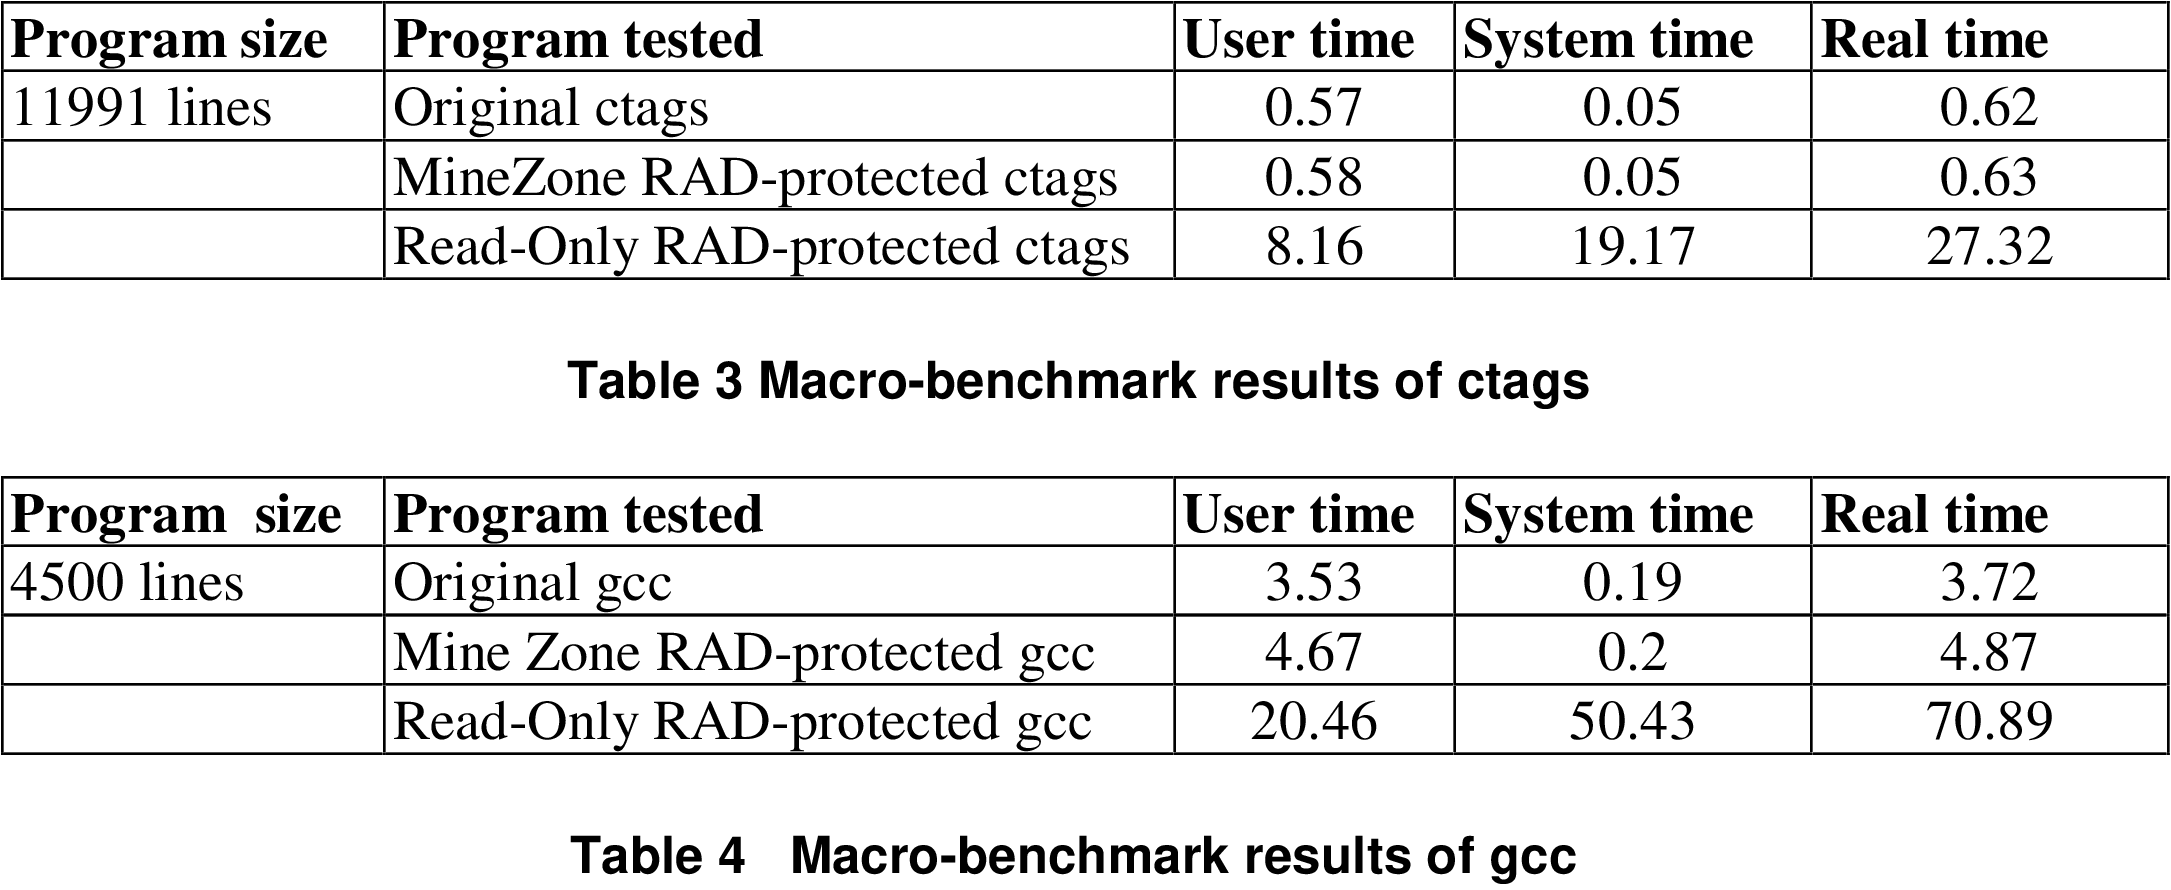
\includegraphics[height=0.8\textheight]{../mitigate/rad-results}
\end{frame}



\subsection{exceptions, setjmp, etc.}
\usetikzlibrary{arrows.meta,patterns}

\begin{frame}{automatic shadow stacks?}
    \begin{itemize}
    \item if we change how CALL/RET works\ldots
    \item \ldots maybe we can add shadow stack support to existing programs?
    \begin{itemize}
        \item either with hardware support, or
        \item in software with emulation techniques?
        \end{itemize}
    \vspace{.5cm}
    \item well, there's a problem\ldots
    \end{itemize}
\end{frame}


\begin{frame}[fragile,label=noAutomaticStack1]{the problem in C++}
\begin{lstlisting}[language=C++,style=smaller]
void Foo() {
    try {
        ... Bar() ...
    } except (std::runtime_error &error) {
        ...
    }
}

void Bar() {
    ... Quux() ...
}
void Quux() {
    ...
    throw std::runtime_error("...");
    ...
}
\end{lstlisting}    
\end{frame}

\begin{frame}[fragile,label=noAutomaticStack2]{the problem in C}
\begin{lstlisting}[language=C++,style=smaller]
jmp_buf env;
const char *error;
void Foo() {
    if (0 == setjmp(env)) {
        Bar();
    } else {
        ...
    }
}

void Bar() {
    ... Quux() ...
}
void Quux() {
    ...
    error = "...";
    longjmp(env, 1);
    ...
}
\end{lstlisting}    
\end{frame}

\begin{frame}{shadow stacks and non-lcoal returns}
    \begin{itemize}
    \item need to modify these functions to support shadow stacks, it seems?
    \item violates idea of hardware extension that modifies CALL/RET operation
    \end{itemize}
\end{frame}

\begin{frame}{one way: dealing with non-local returns}
\begin{itemize}
\item exceptions and setjmp/longjmp deliberately skip return calls
\item one solution: ``direct'' shadow stack
\item fixed (possibly secret) offset from normal stack
\item shadow stack only stores return addreses
    \begin{itemize}
    \item space in between return addresses left as nulls
    \end{itemize}
\end{itemize}
\begin{tikzpicture}[overlay,remember picture]
\coordinate (top) at ([xshift=-5cm,yshift=-2.5cm]current page.north east);
\draw[very thick] (top) rectangle ++(4cm, -7cm);
\draw[thick,pattern=north west lines] (top) ++(0cm, -1cm) rectangle ++(4cm, -2cm) node[yshift=-0.5cm,midway,fill=white] {shadow stack};
\draw[thick,pattern=north west lines] (top) ++(0cm, -4cm) rectangle ++(4cm, -2cm) node[yshift=-0.5cm,midway,fill=white] {normal stack};
\draw[thick,fill=blue!20] (top) ++(0cm, -1.4cm) rectangle  ++(4cm, -0.1cm) coordinate (after shadow ra);
\draw[thick,fill=blue!20] (top) ++(0cm, -4.4cm) rectangle  ++(4cm, -0.1cm) coordinate (after ra);
\draw[thick,fill=blue!20] (top) ++(0cm, -1.1cm) rectangle  ++(4cm, -0.1cm);
\draw[thick,fill=blue!20] (top) ++(0cm, -4.1cm) rectangle  ++(4cm, -0.1cm);
\draw[thick,fill=orange!20] (top) ++(0cm, -4.2cm) rectangle  ++(4cm, -0.2cm);
\draw[thick,fill=orange!20] (top) ++(0cm, -4cm) rectangle  ++(4cm, -0.1cm);
\node[anchor=north,font=\small,fill=white] at ([xshift=-2cm]after shadow ra) {shadow RA};
\node[anchor=north,font=\small,fill=white] at ([xshift=-2cm]after ra) {return addr};
\path[draw,very thick,-Latex] (after ra) -- ++(.25cm,0cm) |- (after shadow ra);
\end{tikzpicture}
\end{frame}


\subsection{exercise: shadow stacks stop}
\begin{frame}{what do shadow stacks stop?}
    \begin{itemize}
    \item combined with a information leak that can dump arbitrary bytes of memory, \\
       which of these exploits would shadow stacks stop\ldots
    \begin{itemize}
    \item A. using format string exploit to point stack return address to the `system' function
    \item B. using format string exploit to point VTable to the `system' function
    \item C. using an unchecked string copy that goes over the end of a stack buffer into the return address and pointing the return address to the `system' function
    \item D. using a buffer overflow that overwrites a saved stack pointer value to cause return to use a different address
    \item E. using pointer subterfuge to overwrite the GOT entry for `printf' to point to the `system' function
    \end{itemize}
    \end{itemize}
\end{frame}


